\documentclass[main.tex]{subfiles}

\begin{document}

\section{Description of the simulation}

A 100 particles interacts with each other through a Lennard-Jones potential with parameters $\epsilon$ and $\sigma$ inside a box modeled using Lennard-Jones potential with sides of $20\sigma$.
The system has an initial temperature $T=2\epsilon/\kappa_{B}$.

\subsection{Equations of motion}

The movement of the particles are going to be describe using Newton's second law of motion and the relation between a force and a conservative potential,
\begin{gather}
    m_{i}\vec{a_{i}} = \sum_{j\neq i}-\grad U_{j\to i}, \label{eqn:movement}
\end{gather}
where $m_{i}\vec{a_{i}}$ is the change in momentum of the particle $i$ and is set to be equal to the sum of the forces applied by a particle $j$ over the particle $i$ through a potential $U$.
Knowing that the interactions between the particles are going to be modeled using the Lennard-Jones potential, $U$ can be expressed as,
\begin{gather}
    U_{j\to i}\qty(r) = 4\epsilon\qty[\qty(\frac{\sigma}{r_{ij}})^{12} - \qty(\frac{\sigma}{r_{ij}})^{6}], \label{eqn:LJpotential}
\end{gather}
where $r_{ij}$ is the distance between the particles $i$ and $j$, $\sigma$ represent a distance in which a repulsive effect is predominant, usually associated with particle size and $epsilon$ is a constant with units of energy [research later the interpretation].

In this case, the force is the derivative of the potential with respect the distance between particles,
\begin{gather*}
    \vec{F}_{j\to i}\qty(r) = \frac{4\epsilon}{r}\qty[ 12\qty(\frac{\sigma}{r_{ij}})^{12} - 6\qty(\frac{\sigma}{r_{ij}})^{6} ]~\hat{r},
\end{gather*}
and the equation\eqref{eqn:movement} can be rewritten as, 
\begin{gather}
    m_{i}\vec{a_{i}} = \frac{4\epsilon}{r}\qty[ 12\qty(\frac{\sigma}{r_{ij}})^{12} - 6\qty(\frac{\sigma}{r_{ij}})^{6} ]~\hat{r}. \label{eqn:movementF}
\end{gather}

With this expression, the force is multiplied by the unit vectors of the distance between the particles to get the the $x$ and $y$ component of the force leading to,
\begin{align}
    m_{i}\vec{a_{xi}} &= \frac{4\epsilon}{r}\qty[ 12\qty(\frac{\sigma}{r_{ij}})^{12} - 6\qty(\frac{\sigma}{r_{ij}})^{6} ]\frac{x_{i}-x_{j}}{r_{ij}}~\hat{x}, \label{eqn:movementFx} \\
    m_{i}\vec{a_{yi}} &= \frac{4\epsilon}{r}\qty[ 12\qty(\frac{\sigma}{r_{ij}})^{12} - 6\qty(\frac{\sigma}{r_{ij}})^{6} ]\frac{y_{i}-y_{j}}{r_{ij}}~\hat{y}. \label{eqn:movementFy}
\end{align}

In the next section it will be explained the implementation of the boundary conditions, the algorithm to establish initial conditions and the numerical method to solve the equations of motion.

% Incrementing the number of particles, the temperature is exact. 

% https://www.researchgate.net/publication/320551421_Mechanical_Behavior_of_Nano_Structures_Using_Atomic-Scale_Finite_Element_Method_AFEM

\subsection{Boundary condition}

To confine the particles in a box with size of $20\sigma$, it is use the Lennard-Jones potential.
In which the variable $r$ is the distance between the particle and the limit of the box, and the parameter $\sigma_{w}$ can be related with the width of the edge of the box.

To simplify the implementation of the force, the potential is evaluate in a one spatial dimension, hence, there are 4 extras forces in the particles due to the boundaries conditions,
\begin{align}
    U_{w_{x}\to i}\qty(r) &= 4\epsilon\qty[\qty(\frac{\sigma_{w}}{x_{i}-w_{x}})^{12} - \qty(\frac{\sigma_{w}}{x_{i}-w_{x}})^{6}], \\
    U_{w_{y}\to i}\qty(r) &= 4\epsilon\qty[\qty(\frac{\sigma_{w}}{y_{i}-w_{y}})^{12} - \qty(\frac{\sigma_{w}}{y_{i}-w_{y}})^{6}].
    %\label{eqn:LJpotential}
\end{align}

\begin{comment}
 Considering that the parameter $\sigma$ is associated with a particle size, this parameter can be re-interpreted as a wall limit and use it to construct a box.
Therefore, a box can be described as,
\begin{gather}
    U_{w\to i}\qty(r) = 4\epsilon\qty[\qty(\frac{20\sigma}{r_{iw}})^{12} - \qty(\frac{20\sigma}{r_{iw}})^{6}], \label{eqn:LJwall}
\end{gather}
and $r_{iw}$ is the distance between the wall and the particle.   
\end{comment}

\subsection{Initial conditions}

Knowing that the potential is proportional to the inverse of the distance between particles is important to set a minimum distance between the particles to avoid infinite values in the force and prevent particles from escaping the box.
For that, the space is partitioned by segments of $1.5\sigma$ of length and the size of the space is reduce by $20\sigma-2\sigma_{w}$ to prevent placing a particle near the wall.
This implementation create an evenly particle placement at the initial condition, as shown in figure \ref{fig:InPos100part}

\begin{figure}[ht!]
    \centering
    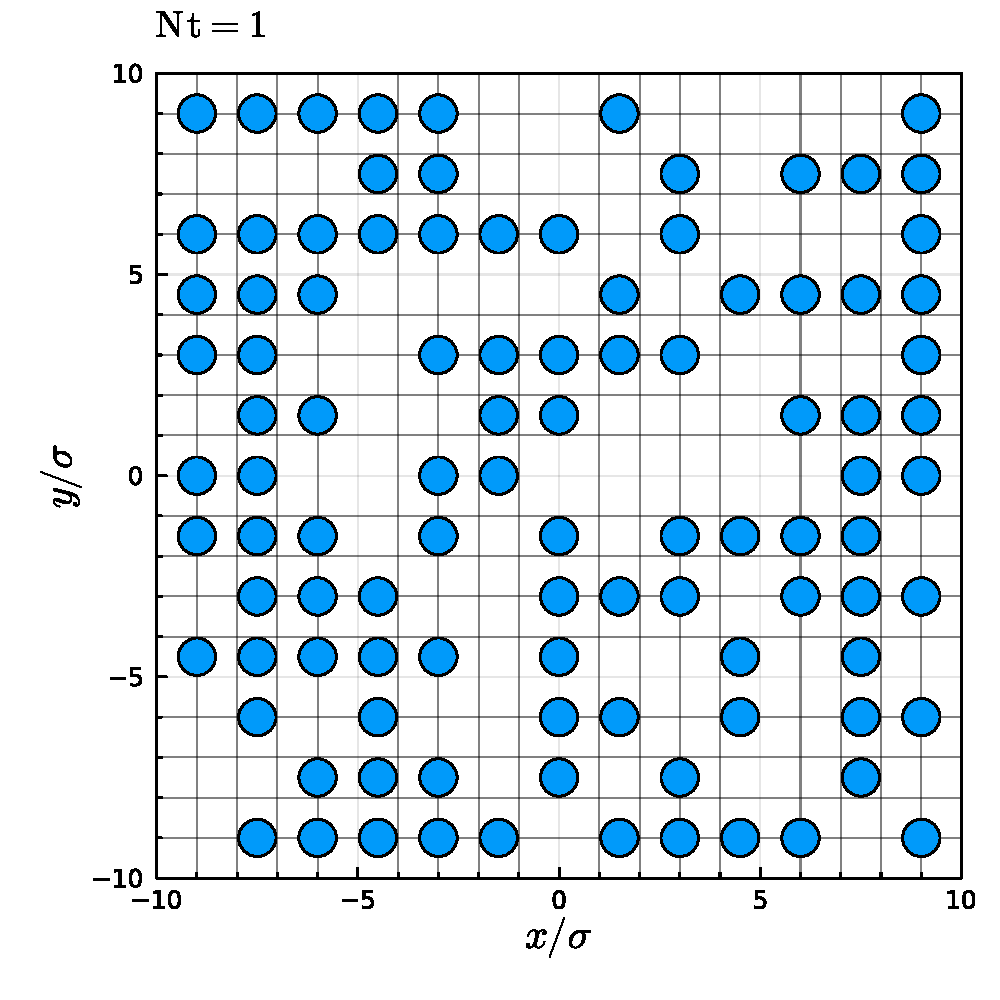
\includegraphics[width=0.7\textwidth]{imgs/hw1/100IniPos.pdf}
    \caption{Initial position for 100 particles uniformly spaced.}
    \label{fig:InPos100part}
\end{figure}

To the set of initial velocities, the Maxwell-Boltzmann distribution for molecular velocity components is used,
\begin{gather}
    P\qty(\upsilon_{x}) = \qty(\frac{m}{2\pi kT})^{1/2}\exp\qty[-\frac{m}{2kT}\upsilon_{x}^{2}],
\end{gather}
which is a normal distribution with standard deviation of $\sqrt{k_{b}T/m}$ and mean $0$.

\subsection{Numerical method}

% https://www2.ph.ed.ac.uk/~dmarendu/MVP/MVP03.pdf
With the boundary and initial conditions set, the equations of movement \eqref{eqn:movementFx},\eqref{eqn:movementFy} can be solved using the Velocity Verlet algorithm,
\begin{align}
    \vec{v_{i}}\qty(t+\Delta t/2) &= \vec{v_{i}}\qty(t) + \frac{\Delta t}{2}\frac{1}{m_{i}}\vec{F_{j\to i}}\qty(\vec{r_{i,j}}\qty(t)), \\
    \vec{r_{i}}\qty(t+\Delta t) &= \vec{r_{i}}\qty(t) + \Delta t \vec{v_{i}}\qty(t+\Delta t/2), \\
    \vec{v_{i}}\qty(t+\Delta t) &= \vec{v_{i}}\qty(t+\Delta t/2) + \frac{\Delta t}{2}\frac{1}{m_{i}}\vec{F_{j\to i}}\qty(\vec{r_{i,j}}\qty(t+\Delta t)).
\end{align}

%The Velocity Verlet algorithm is going to be used to solve the system described by \ref{eqn:Syseqn}.
%The velocity Verlet is a method of 

% https://lamma.engineering.unt.edu/sites/default/files/class5_handout_mtse_5010_2018.pdf

\section{Results}

The numerical method is implemented in Julia and the scripts can be access in the following git-hub repository: \href{https://github.com/FranVT/NanoTech-Masters}{\color{blue}{FranVT Repository}} .
It is important to mention that almost all physical parameters are set to $1$ in all the simulations to simplify the analysis and focus in the overall phenomena of the system, the energy for the innerparticle interaction is equal to $5$, causing a initial temperature of $10$.

In the figure \ref{fig:10PartPlot}
it is shown the trajectories of 10 particles with Nt steps with the purpose of showing the collision with the boundaries, ensuring the correct implementation of the boundary conditions, force and numerical method.
Also, it can be observed the collision between particles and the change of momentumm.

\begin{figure}[ht!]
    \centering
    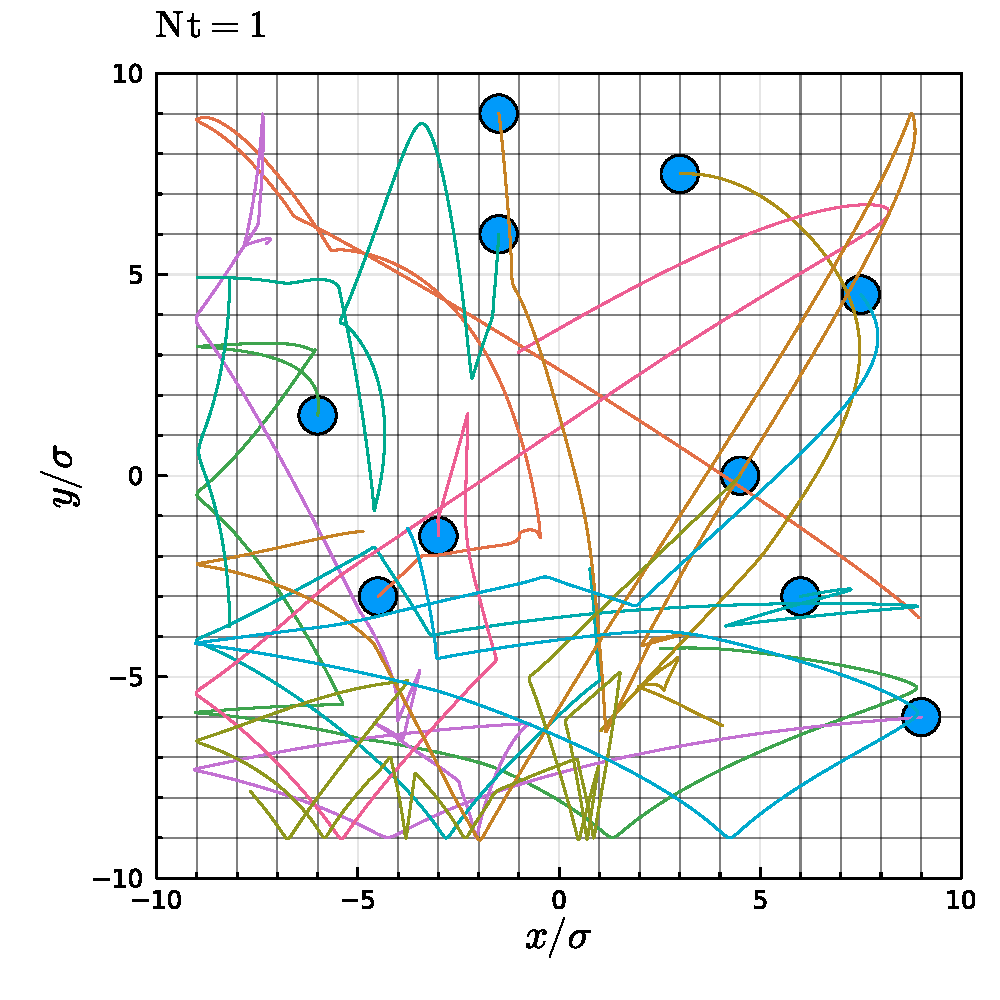
\includegraphics[width=0.7\textwidth]{imgs/hw1/10PartPosition.pdf}
    \caption{Position of 10 particles for Nt steps.}
    \label{fig:10PartPlot}
\end{figure}


Beside the position of the particles, it is useful to observed the evolution of the temperature of the system, which is related with the average kinetic energy of the system by the following equation,
\begin{gather}
    T = \frac{2}{3}\frac{1}{k_{B}}\qty[~\overline{\frac{1}{2}mv^{2}}~]\label{eqn:Temperature}.
\end{gather}

In the figure \ref{fig:temp100PArt} is shown the evolution of the temperature of the system with 100 particles and in the following link \href{https://tecmx-my.sharepoint.com/:i:/g/personal/a00827546_tec_mx/EcEmhXA6lAhGnkAhsRE2kuUBhrXytAb75rOMnJR9yHd_0g?e=JAt8PD}{\color{blue}{Link to the animation}} it can be access and animation of the evolution of the system.
In that gif is shown the time node and the temperature in that time step.

\begin{figure}[ht!]
    \centering
    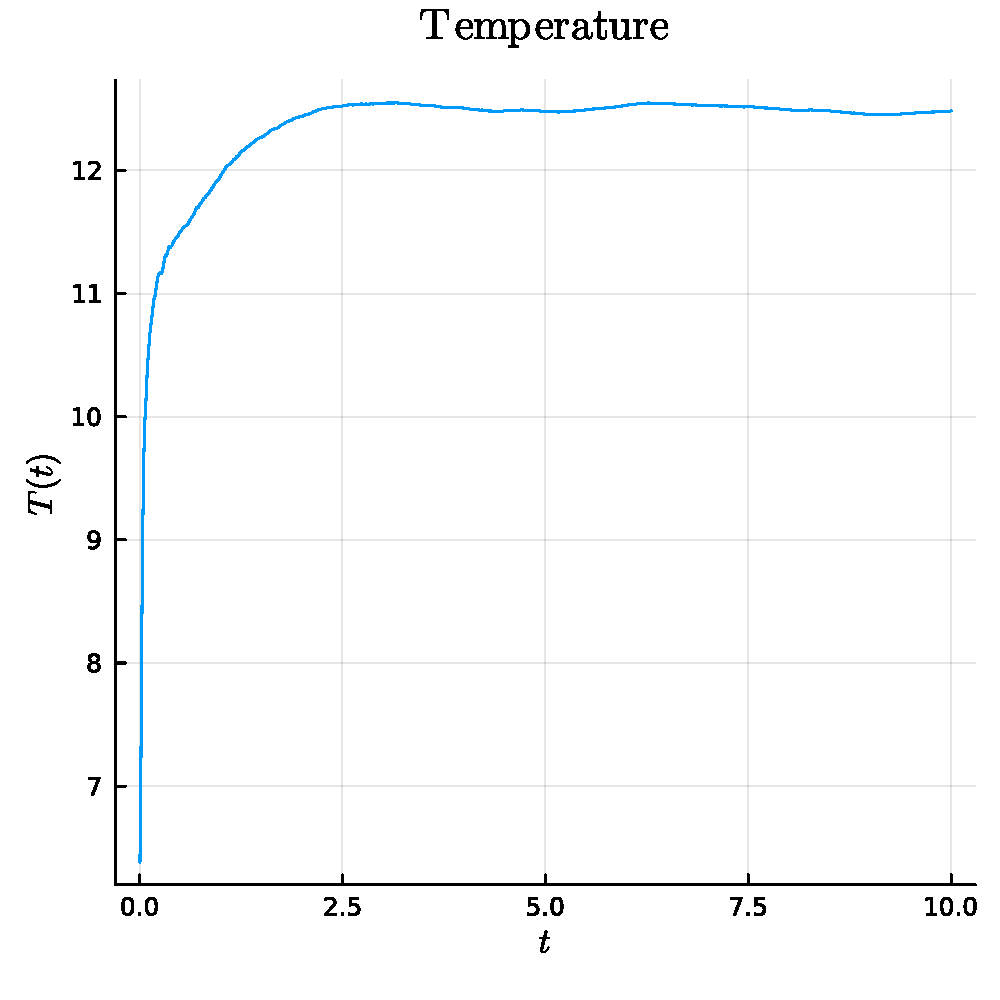
\includegraphics[width=0.7\textwidth]{imgs/hw1/100TempPlot.pdf}
    \caption{Temperature over time froma system of 100 particles}
    \label{fig:temp100PArt}
\end{figure}

Knowing the relation between the temperature and the kinetic energy with equation \eqref{eqn:Temperature}, it is possible to assure that the numerical implementation converges, because the value of the variable oscillates around a constant temperature.
However, that value is above the initial temperature, which is $T=10$, this issue can be related with the quantity of particles and size of the box or the values assign to the physical parameters.

In conclusion, it can be said that a correct implementation of the algorithm of Velocity Verlet to simulate the evolution of a characteristic basic system of molecular dynamics with hard boundary conditions is achieve.
Also, the fact that the evolution of the temperature of the system tends to a constant value shows that the algorithm converges.
Finally,it can be improved the definition of the physical parameters to relate the system with experimental systems.


\end{document}